\documentclass[aps,pra,reprint,amsmath,amssymb,nofootinbib,floatfix]{revtex4-2}
\usepackage[T1]{fontenc}
\usepackage[utf8]{inputenc}
\usepackage{lmodern,amsthm,mathtools}
\usepackage{microtype,graphicx,booktabs}
\usepackage[colorlinks=true,linkcolor=blue,citecolor=blue,urlcolor=blue]{hyperref}
\hypersetup{pdfauthor={Tingyu Zhang and Yan Cen},pdftitle={Sharp reset-error boundaries for time-homogeneous qubit dynamics}}
\newtheoremstyle{aps}{\topsep}{\topsep}{\normalfont}{\parindent}{\itshape}{.}{ }{}
\theoremstyle{aps}
\newtheorem{theorem}{Theorem}
\newtheorem{lemma}[theorem]{Lemma}
\newtheorem{proposition}[theorem]{Proposition}
\newtheorem{corollary}[theorem]{Corollary}
\DeclareMathOperator{\tr}{tr}
\DeclareMathOperator{\diag}{diag}
\newcommand{\Q}{\mathcal Q_2}
\newcommand{\Diss}{\mathcal D}
\newcommand{\eps}{\epsilon}
\newcommand{\pos}[1]{\left[#1\right]_+}
\newcommand{\ket}[1]{|#1\rangle}
\newcommand{\bra}[1]{\langle#1|}
\newcommand{\proj}[1]{|#1\rangle\langle#1|}
\begin{document}
\title{Sharp reset-error boundaries for time-homogeneous qubit dynamics}
\author{Tingyu Zhang}
\email{23300190021@m.fudan.edu.cn}
\author{Yan Cen}
\email[Corresponding author: ]{cenyan@fudan.edu.cn}
\affiliation{Department of Physics, Fudan University, Shanghai, China}




\begin{abstract}
Resetting a qubit with a time-independent Lindblad generator requires considering both the removal of unwanted population from one input and the disturbance of the target input. Quantifying this tradeoff requires optimizing over all generators compatible with the same preparation and measurement basis. For reset toward $\ket1$, let $a=P(0|0)$ and $\eps=P(0|1)$. This paper determines the largest population-order reversal $G(\eps)=\max(\eps-a)$ at fixed actual disturbance $\eps$. As $\eps\downarrow0$, over all qubit Lindblad generators and their probability closure, $G(\eps)\sim(4/e)\eps/\log(1/\eps)$. If the generator admits a stationary state diagonal in the preparation--measurement basis, the sharp law is $G_{\rm diag}(\eps)\sim(64/e^2)\eps/\log^2(1/\eps)$. Explicit single-jump dynamics attain both laws. The different scales arise from direct coherence readout in a tilted stationary eigenbasis and coherence feedback into population, respectively. Every finite-generator sequence saturating the unrestricted law has stationary coherence squared asymptotic to $\eps$ and a purity defect $o(\eps)$. These results quantify the role of stationary coherence in autonomous reset and give sharp endpoint constraints on homogeneous quantum embedding.
\end{abstract}
\maketitle

\section{Introduction}\label{sec:setting}

Autonomous reset prepares a target state using fixed open-system dynamics. For a qubit, the same generator must remove unwanted population from one basis input while limiting the disturbance of the target input. The compatibility of these two conditional probabilities with a time-independent quantum Markov evolution is a homogeneous quantum-embedding problem.

Homogeneous quantum embedding of stochastic matrices was studied by Shahbeigi \emph{et al.}, who obtained analytic exclusion regions and numerical boundary candidates \cite{Shahbeigi2024}. Their four-parameter single-jump family provides a direct antecedent to the attaining dynamics used here. Its numerical success did not establish optimality over all generators. The present contribution is the sharp endpoint boundary of that full class, together with a distinct boundary for generators admitting a diagonal stationary state and necessary stationary-state structure at leading saturation.

The underlying coherence mechanisms have established precedents. Quantum fixed-point reachability can exceed classical population reachability \cite{KorzekwaLostaglio2021}, and classical reductions of quantum dynamics can lose $P$-divisibility as coherence returns information to populations \cite{Benatti2024}. The results below quantify the largest population reversal permitted by a \emph{single time-independent generator} near reset. Section~\ref{sec:model} defines the model and error tradeoff. Section~\ref{sec:results} states the sharp bounds and stationary-state constraints. Sections~\ref{sec:mechanisms} and \ref{sec:universal} give attaining dynamics and universal upper bounds, respectively. Section~\ref{sec:discussion} discusses the physical implications, relation to prior work, and open questions. Section~\ref{sec:conclusions} summarizes the main results.

\section{Model}\label{sec:model}

Prepare a qubit in either $\ket0$ or $\ket1$, apply the same evolution for the same duration, and measure in the same basis. Near reset toward $\ket1$, write the column-stochastic probability table as

\begin{equation}\label{eq:table}
 T(a,1-\eps)=\begin{pmatrix}a&\eps\\1-a&1-\eps\end{pmatrix}.
\end{equation}
Here $a$ is the unwanted output population for the input that needs resetting, and $\eps$ is the disturbance introduced into the target input. Their difference is

\begin{equation}\label{eq:det}
 q:=a-\eps=\det T.
\end{equation}
For a diagonal input with unwanted population $r$, linearity gives
\begin{equation}\label{eq:population-order}
 \rho_r=r\proj0+(1-r)\proj1,\qquad
 P_0(r)=\eps+(a-\eps)r.
\end{equation}
Thus $q<0$ means that an input with more unwanted population ends with less of it. The question is how large this reversal can be when the dynamics is generated by one fixed qubit Lindbladian.

Fixing the \emph{actual measured} $\eps$ selects a slice of the homogeneous-embedding region. For a realized reversal $\Delta=\eps-a>0$, the worst population error among diagonal inputs remains $\eps$, while the equally weighted error is $\eps-\Delta/2$. The task therefore concerns input-conditioned population data. If one instead imposed only an allowance $\eps\le\delta$ with unrestricted time and rates, ordinary damping to $\ket1$ could already approach perfect reset with $\eps=0$. The two measured probabilities also leave the response to coherent inputs unspecified.

The model includes all time-independent Gorini--Kossakowski--Sudarshan--Lindblad generators \cite{GKS1976,Lindblad1976}

\begin{equation}\label{eq:gksl}
 \begin{gathered}
 \mathcal L(\rho)=-i[H,\rho]+\sum_\mu\Diss[J_\mu](\rho),\\
 \Diss[J](\rho)=J\rho J^\dagger-\tfrac12\{J^\dagger J,\rho\},
 \end{gathered}
\end{equation}
on $\mathbb C^2$, with a Hermitian Hamiltonian and a finite collection of finite jump matrices. The system has no auxiliary levels, and the preparation and measurement basis is fixed throughout. Rates, duration, and Hamiltonian strength are unrestricted.

Identify each table $T(a,1-\eps)$ with the pair $(a,1-\eps)$. Let $\mathcal Q_2^{\rm fin}$ be the tables obtained from $e^{t\mathcal L}$ at finite $t\ge0$, and set

\begin{equation}\label{eq:closure}
 \Q=\overline{\mathcal Q_2^{\rm fin}}\subset[0,1]^2.
\end{equation}
This is the arbitrary-accuracy convention of Ref.~\cite{Shahbeigi2024}: each approximant has finite parameters, but no common rate or time bound is required. The rescaling $H\mapsto tH$, $J_\mu\mapsto\sqrt tJ_\mu$ fixes the observation time at one without excluding singular parameter sequences.

At fixed actual disturbance define

\begin{equation}\label{eq:G}
 G(\eps)=\max\{\eps-a:(a,1-\eps)\in\Q\}.
\end{equation}
The maximum exists because $\Q$ is compact. Its fiber is nonempty: classical relaxation to population $\eps$ gives $a=\eps$ in the closure. In particular $0\le G(\eps)\le\eps$.

Let $\mathcal Q_{\rm diag}$ be the probability closure of finite realizations whose generator admits at least one stationary state diagonal in the preparation--measurement basis. This permits transient coherence and population--coherence coupling; it assumes neither a unique stationary state nor preservation of all diagonal states. Define $G_{\rm diag}$ by \eqref{eq:G} with $\Q$ replaced by $\mathcal Q_{\rm diag}$.

\section{Reset-error bounds}\label{sec:results}\label{sec:diagonal}

The two classes have different asymptotic boundaries near perfect reset.

\begin{theorem}[Sharp autonomous reset law]\label{thm:main}
For the full time-independent qubit GKSL probability closure,
\begin{equation}\label{eq:main}
 \lim_{\eps\downarrow0}\frac{\log(1/\eps)}{\eps}G(\eps)=\frac4e.
\end{equation}
Equivalently, the lower reset boundary is
\begin{equation}\label{eq:boundary}
 \min\{a:(a,1-\eps)\in\Q\}
 =\eps\left[1-\frac{4/e+o(1)}{\log(1/\eps)}\right].
\end{equation}
\end{theorem}

\begin{theorem}[Diagonal-stationary-state law]\label{thm:diagonal}
The restricted class has the sharp endpoint asymptotic
\begin{equation}\label{eq:diagonal-law}
 G_{\rm diag}(\eps)=\left(\frac{64}{e^2}+o(1)\right)
 \frac\eps{\log^2(1/\eps)}.
\end{equation}
\end{theorem}

Both laws imply $a/\eps\to1$ at the optimal boundary: the two input-conditioned errors agree to leading order, while the smaller difference $\eps-a$ records the quantum population reversal. Its relative size vanishes in the perfect-reset limit.

The two laws fit between classical dynamics and time-dependent quantum control:
\begin{equation}\label{eq:three}
 \begin{aligned}
 G_{\rm cl}(\eps)&=0,&
 G_{\rm diag}(\eps)&\sim\frac{64}{e^2}\frac{\eps}{\log^2(1/\eps)},\\
 G(\eps)&\sim\frac4e\frac{\eps}{\log(1/\eps)},&
 G_{\rm td}(\eps)&=\eps.
 \end{aligned}
\end{equation}
Here $G_{\rm cl}$ and $G_{\rm td}$ use the same fixed-error optimization and probability-closure convention for classical two-state dynamics and time-dependent qubit GKSL control, respectively. Even for time-dependent classical rates,
$q(t)=\exp[-\int_0^t(k_{01}(s)+k_{10}(s))\,ds]\ge0$.
Time-dependent qubit GKSL control permits all two-state stochastic tables \cite{KorzekwaLostaglio2021}. These comparisons use the same system dimension, basis, and probability task.

The unrestricted leading optimum also constrains every stationary state of an attaining sequence. For realizations with $a\le\eps$ sufficiently small, every stationary state can be written in its eigenbasis as

\begin{equation}\label{eq:stationary}
 \begin{gathered}
 \rho_*=\nu\proj e+(1-\nu)\proj g,\\
 0\le\nu<\tfrac12,\qquad p=|\langle0|g\rangle|^2.
 \end{gathered}
\end{equation}
\begin{corollary}[Stationary-state saturation]\label{cor:saturation}
Consider a sequence of finite qubit GKSL realizations with actual errors $a_n,\eps_n$, where $\eps_n\downarrow0$ and
\begin{equation}\label{eq:saturation}
 \frac{\log(1/\eps_n)}{\eps_n}(\eps_n-a_n)\longrightarrow\frac4e.
\end{equation}
For each sufficiently large $n$, choose any stationary state and let $\nu_n,p_n$ be as in \eqref{eq:stationary}. Then
\begin{equation}\label{eq:rigidity}
 \frac{\nu_n}{\eps_n}\longrightarrow0,
 \qquad\frac{p_n}{\eps_n}\longrightarrow1.
\end{equation}
\end{corollary}
In the fixed measurement basis this gives
\begin{equation}\label{eq:coherence-purity}
 \begin{gathered}
 \left|\bra0\rho_{*,n}\ket1\right|^2
 =(1-2\nu_n)^2p_n(1-p_n)\sim\eps_n,\\
 1-\tr(\rho_{*,n}^2)=2\nu_n(1-\nu_n)=o(\eps_n).
 \end{gathered}
\end{equation}
The stationary coherence tends to zero, but its square uses the leading population-error budget. Mixedness cannot occupy a nonzero fraction of that budget. This is a necessary structure along finite realizations, not a prescribed generator for an abstract closure point. Its proof is given in Section~\ref{sec:universal}.

\begin{equation}\label{eq:ratio}
 \frac{G_{\rm diag}(\eps)}{G(\eps)}
 \sim\frac{16}{e\log(1/\eps)}\longrightarrow0.
\end{equation}
Consequently any finite-generator sequence for which
$\liminf\log(1/\eps)(\eps-a)/\eps>0$
eventually admits no stationary state diagonal in the measurement basis: a contrary subsequence would satisfy Theorem~\ref{thm:diagonal} and have vanishing scaled gain. Stationary coherence is necessary for a nonvanishing fraction of the unrestricted leading scale; transient coherence alone can still realize the smaller scale.



\section{Asymptotically optimal constructions}\label{sec:mechanisms}

The two bounds are attained by different routes from population through coherence. Figure~\ref{fig:gain-comparison} compares explicit realizations at the same \emph{actual} $\eps$ on a common scale. These are constructive lower bounds; their finite-error ordering need not coincide with the ordering of the optimized classes.

\begin{figure}[tbp]
 \centering
 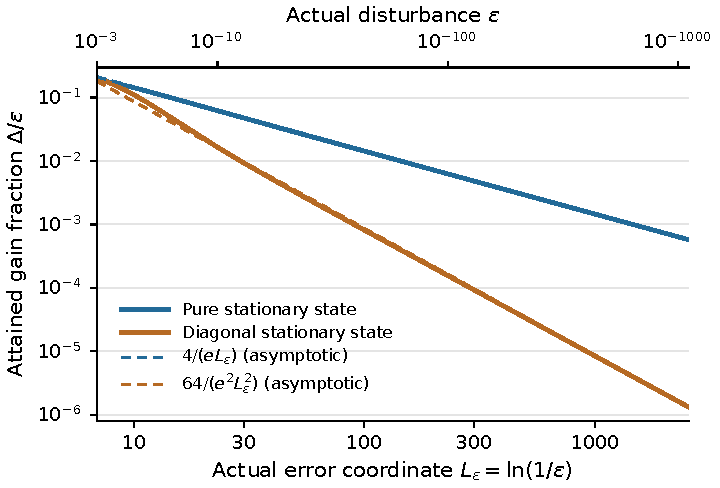
\includegraphics[width=\columnwidth]{reset_gain_comparison.pdf}
 \caption{Population-order reversal at the same actual disturbance $\eps=P(0|1)$, shown as $\Delta/\eps$ with $\Delta=\eps-a$. Solid curves are the tilted pure-state construction, Eqs.~\eqref{eq:familyparams}--\eqref{eq:familyjump}, and diagonal-state construction, Eqs.~\eqref{eq:diag-jump}--\eqref{eq:diag-xstar}. Dashed curves are their leading laws $4/(eL_\eps)$ and $64/(e^2L_\eps^2)$, where $L_\eps=\log(1/\eps)$. Solid curves give attainable lower bounds for the corresponding optimal gains. The diagonal construction exceeds the displayed pure-state construction at $\eps=10^{-3}$; the hierarchy of Theorems~\ref{thm:main} and \ref{thm:diagonal} holds asymptotically.}
 \label{fig:gain-comparison}
\end{figure}

\subsection{Tilted pure stationary state}

For a stationary eigenvector with $p=|\langle0|g\rangle|^2$, use the readout coefficients
\begin{equation}\label{eq:vw}
 \begin{gathered}
 v=1-2p,\qquad w=2\sqrt{p(1-p)},\\
 V=v^2,\quad W=w^2,\quad R=vw.
 \end{gathered}
\end{equation}
Let $L\to\infty$ and define
\begin{equation}\label{eq:familyparams}
 p=e^{-L},\qquad A=L+\log L+1-\log4,\qquad B=A/L.
\end{equation}
Choose orthonormal vectors
\begin{equation}\label{eq:familybasis}
 \ket g=\sqrt p\ket0+\sqrt{1-p}\ket1,\qquad
 \ket e=\sqrt{1-p}\ket0-\sqrt p\ket1,
\end{equation}
In the ordered basis $(e,g)$, take a single jump and no Hamiltonian:
\begin{equation}\label{eq:familyjump}
 J=\begin{pmatrix}-\sqrt B&0\\\sqrt A&0\end{pmatrix},\qquad H=0.
\end{equation}
For every sufficiently large finite $L$, this generator has the stationary state $\proj g$. For a state $\rho$, define its population $n=\bra e\rho\ket e$ and coherence $z=\bra e\rho\ket g$. The measured population is $P_0=p+vn+w\operatorname{Re}z$, and the dynamics obeys
\begin{equation}\label{eq:triangular}
 \dot n=-An,\qquad
 \dot z=-\sqrt{AB}\,n-\Gamma z,\qquad \Gamma=(A+B)/2.
\end{equation}
Set
\begin{equation}\label{eq:familykernels}
 \begin{gathered}
 F=e^{-A},\qquad S=e^{-\Gamma},\\
 J_0=\int_0^1e^{-At}e^{-\Gamma(1-t)}\,dt
 =\frac{S-F}{A-\Gamma}.
 \end{gathered}
\end{equation}
For the difference of the two input states, let $u$ and $z$ denote the differences of these population and coherence coordinates. Then $q=vu+w\operatorname{Re}z$, with $(u(0),z(0))=(v,w)$, and direct solution gives
\begin{equation}\label{eq:familyq}
 q=v^2F+w^2S-vw\sqrt{AB}\,J_0.
\end{equation}
For the actual input $\ket1$, the initial population and coherence are $n(0)=p$, $z(0)=-w/2$, so its actual error is
\begin{equation}\label{eq:actualepsilon}
 \eps(L)=p+vpF-\frac{w^2}{2}S-pw\sqrt{AB}\,J_0.
\end{equation}
In \eqref{eq:familyq}, the surviving population and coherence terms are positive, while transfer from population to coherence produces the negative cross term. The small inclination of the stationary eigenbasis allows this coherence to enter the population measurement directly. With $A\sim L$, $B/A=1/L$, and $\eps\sim e^{-L}$, the cross term has twice the magnitude of the surviving population term at leading order, giving
$\Delta\sim(4/e)\eps/\log(1/\eps)$.
Appendix~\ref{app:unrestricted-sharpness} gives the explicit expansions and proves that the family covers every sufficiently small positive actual $\eps$.

The displayed GKSL representation has $H=0$; the jump itself contains coherent amplitudes. Since identity shifts of jumps redistribute terms between the dissipator and Hamiltonian, this representation does not assert the absence of coherent physical resources.

The construction can also keep the jump strength finite. With the operator norm $\|J\|^2=A+B$, fix any rate $\kappa>0$ and rescale
\begin{equation}\label{eq:fixed-strength}
 \begin{gathered}
 J_{\rm phys}=\sqrt{\frac{\kappa}{A+B}}J,\\
 t_{\rm phys}=\frac{A+B}{\kappa}
 \\=\frac{\log(1/\eps)+\log\log(1/\eps)+O(1)}{\kappa}.
 \end{gathered}
\end{equation}
This gives the same channel with $\|J_{\rm phys}\|^2=\kappa$. The direction of the stationary state and the ratio $B/A$ still depend on the target error; each selected generator remains fixed during its evolution.

\subsection{Diagonal stationary state}

When $\rho_*=\diag(\nu,1-\nu)$ in the measurement basis, stationarity gives
\begin{equation}\label{eq:diagonal-exact}
 a=\nu+(1-\nu)q,\qquad \eps=\nu(1-q).
\end{equation}
For $q=-\Delta<0$, these relations become
\begin{equation}\label{eq:overshoot}
 \nu-a=(1-\nu)\Delta,\qquad \eps-\nu=\nu\Delta.
\end{equation}
The input $\ket0$ transiently falls below the stationary unwanted population, while the target input ends slightly above it. A classical two-state relaxation cannot cross its stationary population.

For the two-input difference $\delta\rho$ in the measurement basis, let $u=\delta\rho_{00}$ and $z=\delta\rho_{01}$. An explicit single jump and Hamiltonian keep $z$ real and realize
\begin{equation}\label{eq:diag-real}
 \frac d{dt}\binom uz=
 \begin{pmatrix}-\alpha&r_0\\-c_0&-\lambda_+\end{pmatrix}\binom uz,
 \qquad\lambda_+=\frac{A(1+\chi)^2+B}{2},
\end{equation}
where $\chi=\sqrt{\nu/(1-\nu)}$ and $\alpha,r_0,c_0,\lambda_+>0$; the explicit GKSL realization and coefficients are specified in Appendices~\ref{app:stationary} and \ref{app:diagonal}. The input difference starts at $(u,z)=(1,0)$ and the measured determinant is $q=u(1)$. Population first creates coherence through $-c_0u$, and the coherence then feeds back through $r_0z$. The negative feedback can transiently reverse the population difference even though the stationary coherence is zero.

For the asymptotically optimal constructions, $\tau=B/A$ is of order $1/\log(1/\eps)$. In this regime, the negative slow-mode amplitude is $8\sqrt\nu\,\tau$ to leading order, compared with $4\sqrt{p\tau}$ for direct readout in the tilted pure-state construction. The competing positive population mode decays about twice as fast. To leading order, optimizing their difference gives one quarter of the squared slow-mode amplitude, multiplied by $e^{-\tau L}$. This factor comes from the $O(\tau)$ correction to the slow-to-fast decay-rate ratio $1/2$, with $L=\log(1/\nu)$ or $\log(1/p)$, respectively. The leading gains are therefore $16\nu\tau^2e^{-\tau L}$ and $4p\tau e^{-\tau L}$, with maxima at $\tau L=2$ and $\tau L=1$. The extra factor of $\tau$ explains the additional inverse logarithm. Appendix~\ref{app:diagonal} proves the uniform bound over the full restricted class and gives a matching GKSL realization. In particular, the matching family has
$\nu-a\sim(64/e^2)\nu/\log^2(1/\nu)$.

A diagonal stationary state still permits transient coherence: the term $-c_0u$ creates it immediately. The distinction between stationary coherence and this transient feedback is the physical separation measured by the two theorems.



\section{Universal upper bounds}\label{sec:universal}

To establish optimality of the constructions, the upper-bound argument starts from an arbitrary generator. A constraint on its stationary states controls the error budget, and a population--coherence comparison bounds the largest possible transient reversal.

\subsection{Stationary-state constraint}

Every finite-dimensional GKSL generator has a stationary density matrix; a convergent subsequence of long-time averages of any orbit supplies one. For any fixed point $\rho_*$ of the channel $\Phi=e^{\mathcal L}$, set $p_*=\bra0\rho_*\ket0$. The positive effect $\Phi^*(\proj0)$ has diagonal entries $a,\eps$, hence its off-diagonal entry is bounded by $\sqrt{a\eps}$. Positivity of $\rho_*$ and stationarity give
$p_*\le(\sqrt{ap_*}+\sqrt{\eps(1-p_*)})^2$, and therefore
\begin{equation}\label{eq:budget-cross}
 [(1-\sqrt a)^2+\eps]p_*\le\eps.
\end{equation}
With \eqref{eq:stationary}, $p_*=\nu+(1-2\nu)p$. In the relevant region $a\le\eps\downarrow0$, the exact inversion in Appendix~\ref{app:stationary} yields
\begin{equation}\label{eq:budget-leading}
 p+\nu\le\varrho(\eps)=\eps[1+O(\sqrt\eps)].
\end{equation}
Both stationary inclination and mixedness consume the same small measured-error budget. Replacing a mixed stationary state by a pure one at this point would incur an uncontrolled error on the finer scale $\eps/\log(1/\eps)$.

\subsection{Population--coherence comparison}

In an arbitrary stationary eigenbasis, set $u=\bra e\rho\ket e-\nu$ and $z=\bra e\rho\ket g$. Their homogeneous equations have the form
\begin{equation}\label{eq:core-system}
 \dot u=-\alpha u+\operatorname{Re}(R_0z^*),\qquad
 \dot z=\widetilde C u+Ez^*-(\Gamma+i\omega)z.
\end{equation}
Appendix~\ref{app:stationary} derives these equations for arbitrary jump collections and Hamiltonians, with the exact coefficients in \eqref{eq:ueq}--\eqref{eq:zeq}. In particular, both population feedback and conjugate-coherence coupling are retained.

The frequency term $-i\omega z$ makes no direct contribution to the derivative of $|z|$, so the resulting comparison estimate is uniform in $\omega$. Gram positivity supplies nonnegative bounds $r_0,c_0$ on the coupling strengths and a lower bound $\lambda$ on coherence damping. They define a comparison matrix
$K=\bigl(\begin{smallmatrix}-\alpha&r_0\\c_0&-\lambda\end{smallmatrix}\bigr)$
with nonnegative off-diagonal entries; its parameters are given in \eqref{eq:comparison-coeff}. Choose the relative phase of $e,g$ so that the off-diagonal entry of $\proj0$ is nonnegative. The same equations govern the input difference, with $(u(0),z(0))=(v,w)$ and $q=vu+w\operatorname{Re}z$, using \eqref{eq:vw}. Retaining the population's positive free decay gives
\begin{equation}\label{eq:comparison}
 q(t)\ge 2Ve^{-\alpha t}
 -(v,w)e^{tK}\binom vw\qquad(t\ge0).
\end{equation}

The proof in Appendix~\ref{app:stationary} uses a positive comparison for $|u|,|z|$ followed by the population variation-of-constants formula. This preserves the positive term that competes with the negative coherence transient.

The rate parameters $A,B$ are defined in \eqref{eq:coefficients} from the jump entries in a stationary basis, after setting their $gg$ entries to zero by an identity shift. They reduce to the rates in \eqref{eq:familyjump} for the pure-state construction. At time one, define
\begin{equation}\label{eq:envelope}
 \begin{gathered}
 \mathcal E(p,\nu,A,B)
 =\pos{(v,w)e^K\binom vw-2Ve^{-\alpha}},
 \\ [x]_+=\max(x,0).
 \end{gathered}
\end{equation}
Then $(\eps-a)_+\le\mathcal E$. This enlarged positive system is an upper-bound tool, not an assumed physical generator.

\begin{proposition}[Sharp uniform envelope]\label{prop:envelope}
Let $p,\nu\ge0$, $p+\nu\le\rho$, and $A,B\ge0$. With the definitions above, as $\rho\downarrow0$,
\begin{equation}\label{eq:refined}
 \mathcal E(p,\nu,A,B)
 \le\frac{4p/e+o(\rho)}{\log(1/\rho)}.
\end{equation}
The remainder is a function of $\rho$ alone and is uniform in all four parameters.
\end{proposition}

In the only leading rate-ratio window, put $\tau=B/A$ and $L=\log(1/\rho)$. Exact optimization of the overall rate and the budget $p+\nu\le\rho$ give
\begin{equation}\label{eq:leading-core}
 \mathcal E\le[4p+o(\rho)]\tau e^{-\tau L}
 \le\frac{4p/e+o(\rho)}L.
\end{equation}
The factor $\tau e^{-\tau L}$ peaks at $\tau L=1$. Appendix~\ref{app:envelope} proves this estimate uniformly and controls all remaining ratios, including zero rates, repeated eigenvalues, and arbitrarily large rates. Those other regions contribute $o(\rho/L)$. No bounded-frequency or compact-generator reduction is used.

\subsection{Sharp asymptotics and saturation}

For a finite realization with $a\le\eps$, choose any stationary state. Lemma~\ref{lem:budget} gives $p+\nu\le\varrho(\eps)$, and Lemma~\ref{lem:comparison} and Proposition~\ref{prop:envelope} then yield
\begin{equation}\label{eq:physicalupper}
 \eps-a\le\frac{4p/e+o(\varrho(\eps))}{\log(1/\varrho(\eps))}
 \le\left(\frac4e+o(1)\right)\frac\eps{\log(1/\eps)}.
\end{equation}
The last step uses $\varrho(\eps)=\eps[1+O(\sqrt\eps)]$. If $a>\eps$, the upper bound is immediate.

For clarity, the uniform statement means that for every $\delta>0$ there is $\eps_\delta>0$ such that every finite generator obeys
\begin{equation}\label{eq:finiteuniform}
 \eps-a\le\left(\frac4e+\delta\right)
 \frac\eps{\log(1/\eps)}\qquad(0<\eps<\eps_\delta).
\end{equation}
Fix a probability-closure point with $0<\eps<\eps_\delta$ and approximate it by finite realizations. The approximants eventually lie within the same error interval, and the right-hand side is continuous in $\eps$. Passing to the limit proves \eqref{eq:finiteuniform} for $\Q$. This uses no compactness of generators, stationary-state choices, or decay rates.

The pure-stationary-state construction of Section~\ref{sec:mechanisms}, with the actual-error and continuity arguments in Appendix~\ref{app:unrestricted-sharpness}, supplies the matching lower bound and completes Theorem~\ref{thm:main}. The refined coefficient $4p/e$ also proves Corollary~\ref{cor:saturation}:

\begin{proof}
For all sufficiently large $n$, $a_n<\eps_n$. The budget gives
$p_n+\nu_n\le\eps_n[1+o(1)]$. The refined first inequality of \eqref{eq:physicalupper}, multiplied by $\log(1/\eps_n)/\eps_n$, and \eqref{eq:saturation} force $\liminf p_n/\eps_n\ge1$. Both limits follow from nonnegativity and the budget.
\end{proof}
The coherence and purity identities in \eqref{eq:coherence-purity} follow directly from the stationary eigenvalues and the overlap $p_n$.

For the diagonal class, $p=0$ leaves only round-trip feedback. Appendix~\ref{app:diagonal} refines the signed comparison to the scale $\nu/\log^2(1/\nu)$, proves a uniform bound over every rate ratio, and constructs a matching GKSL generator. Equation~\eqref{eq:diagonal-exact} then converts $\nu$ to the actual $\eps$, and the same probability-closure argument completes Theorem~\ref{thm:diagonal}.



\section{Discussion}\label{sec:discussion}

The two reset laws constrain the conditional population probabilities compatible with one fixed generator. Their logarithmic restriction comes from the requirement of autonomous evolution: time-dependent control can first damp toward $\ket0$, leaving population $\eps$ in $\ket1$ for input $\ket1$, and then apply a unitary swap. This gives $a=0$ and $P(0|1)=\eps$. Thus, in the same two-state system and preparation--measurement basis, time-dependent control reaches $G_{\rm td}(\eps)=\eps$, while a fixed generator reaches only a vanishing fraction of this value.

For a fixed generator, the two scales distinguish direct coherence readout from coherence feedback into population. The diagonal-stationary-state law quantifies transient overshoot beyond classical relaxation \cite{KorzekwaLostaglio2021,Benatti2024}. Transient coherence suffices for reversal on this smaller scale. Leading saturation of the unrestricted law additionally requires squared stationary coherence to exhaust the population-error budget while the relative purity defect vanishes. This necessary condition applies to every stationary state along an asymptotically optimal sequence of finite GKSL realizations.

The attaining families are realized within the earlier four-parameter ansatz or its probability closure. The ansatz uses $H=X$, where $X$ is the Pauli $x$ matrix, and a rank-one jump between states $(\cos\theta,i\sin\theta)^T$ \cite{Shahbeigi2024}. The pure-state family lies in its probability closure, and the diagonal-state family belongs to it exactly at sufficiently small error. Appendix~\ref{app:prior-family} gives the transformations. Their endpoint optimality follows from the full-class upper bounds.

The earlier exclusion gives $a\ge(\eps/2)^{10}[1+o(1)]$ near reset, whereas Theorem~\ref{thm:main} determines $a/\eps\to1$ and its leading correction. Appendix~\ref{app:exclusions} identifies the additional excluded region $\eps/2<a<3\eps/4$ for sufficiently small $\eps$.

The finite-error optimal curve, uniform higher-order corrections, and the boundary away from reset remain open.

\section{Conclusions}\label{sec:conclusions}

The sharp endpoint asymptotics of the reset-error boundary are determined for a single time-independent qubit GKSL generator. At fixed actual disturbance $\eps$, the largest population-order reversal obeys $G(\eps)\sim(4/e)\eps/\log(1/\eps)$ and falls to $G_{\rm diag}(\eps)\sim(64/e^2)\eps/\log^2(1/\eps)$ when the generator admits a stationary state diagonal in the measurement basis. Universal upper bounds and explicit single-jump constructions establish both laws. Leading saturation of the unrestricted law also fixes the stationary coherence and purity scales, connecting the observable error boundary to the stationary-state structure required to attain it.

\begin{acknowledgments}
[Acknowledgments and funding information to be added.]
\end{acknowledgments}

\appendix

\section{Stationary-state reduction}\label{app:stationary}\label{sec:comparison}

\subsection{Stationary-state constraint}

Every finite-dimensional GKSL generator has a stationary density matrix. Indeed, time-average any orbit; a convergent subsequence exists by compactness, and
$\mathcal L(t^{-1}\int_0^t e^{s\mathcal L}(\rho)\,ds)
=(e^{t\mathcal L}(\rho)-\rho)/t\to0$.
The next observation constrains every such state using only the two measured errors.

\begin{lemma}[Stationary error budget]\label{lem:budget}
Let $\Phi$ be a qubit channel with the probabilities in \eqref{eq:table}. For any fixed point $\rho_*$ of $\Phi$, write $p_* =\bra0\rho_*\ket0$. Then the inequality \eqref{eq:budget-cross} holds.
If $a\le\eps<1/4$, diagonalize
$\rho_*$ as in \eqref{eq:stationary}.
Then $p,\nu<1/2$ and
\begin{align}
 p_*&=\nu+(1-2\nu)p,\label{eq:pstar}\\
 p+\nu&\le\varrho(\eps):=1-\sqrt{1-2b_*(\eps)},\nonumber\\
 b_*(\eps)&=\frac{\eps}{1-2\sqrt\eps+2\eps},\label{eq:rhoepsilon}\\
 \varrho(\eps)&=\eps[1+O(\sqrt\eps)].\nonumber
\end{align}
\end{lemma}

\begin{proof}
The positive effect $F=\Phi^*(\proj0)$ has diagonal entries $a,\eps$, so $|F_{01}|\le\sqrt{a\eps}$. Positivity of $\rho_*$ similarly bounds its off-diagonal entry. Since $\Phi(\rho_*)=\rho_*$,
\[
 p_*=\tr(F\rho_*)
 \le\bigl(\sqrt{ap_*}+\sqrt{\eps(1-p_*)}\bigr)^2.
\]
Taking square roots and rearranging proves \eqref{eq:budget-cross}. For $a\le\eps<1/4$, it gives $p_*\le b_*(\eps)<1/2$. Equation~\eqref{eq:pstar} implies $\nu\le p_*$ and $p\le p_*$, so $s=p+\nu<1$. Since
\[
 p_*=s-2\nu p\ge s-\frac{s^2}{2},
\]
and the right-hand side increases on $[0,1)$, inversion yields \eqref{eq:rhoepsilon}.
\end{proof}

\subsection{Population--coherence dynamics}

Fix an arbitrary stationary state and use its eigenbasis $(e,g)$ from \eqref{eq:stationary}. Subtracting each jump's $gg$ entry times the identity, and making the corresponding Hamiltonian adjustment, preserves the generator and gives
\begin{equation}\label{eq:gauge}
 J_\mu=\begin{pmatrix}x_\mu&y_\mu\\z_\mu&0\end{pmatrix},\qquad
 H=\begin{pmatrix}\omega/2&h\\h^*&-\omega/2\end{pmatrix}.
\end{equation}
An irrelevant scalar multiple of the identity has also been removed from $H$. Define
\begin{align}\label{eq:coefficients}
 A&=\sum_\mu|z_\mu|^2,& B&=\sum_\mu|x_\mu|^2,&
 U&=\sum_\mu|y_\mu|^2,\nonumber\\
 C&=\sum_\mu x_\mu z_\mu^*,&
 D&=\sum_\mu x_\mu^*y_\mu,&
 E&=\sum_\mu y_\mu z_\mu^*.
\end{align}
They form the Gram matrix
\begin{equation}\label{eq:gram}
 \begin{pmatrix}B&D^*&C\\D&U&E\\C^*&E^*&A\end{pmatrix}\succeq0,
\end{equation}
whose principal minors imply
$|C|\le\sqrt{AB}$, $|D|\le\sqrt{BU}$, and $|E|\le\sqrt{AU}$.
The stationary equations give exactly
\begin{equation}\label{eq:stationarity}
 U=\frac{A\nu}{1-\nu},\qquad
 h=-i\frac{\nu C-D/2}{1-2\nu}.
\end{equation}
No restriction on the real frequency $\omega$ follows or is imposed.

Let $u=\bra e\rho\ket e-\nu$ be the $\ket e$ population relative to stationarity and $z=\bra e\rho\ket g$ the coherence. Direct substitution in \eqref{eq:gksl} gives
\begin{align}
 \dot u&=-(A+U)u+\operatorname{Re}(R_0z^*),\label{eq:ueq}\\
 \dot z&=\widetilde C u+Ez^*-(\Gamma+i\omega)z,\label{eq:zeq}\\
 \widetilde C&=\frac{C-D}{1-2\nu},\nonumber\\
 R_0&=\frac{2[(1-\nu)D-\nu C]}{1-2\nu},\nonumber\\
 \Gamma&=\frac{A+B+U}{2}.\nonumber
\end{align}
The same homogeneous equations govern the difference between two trajectories. Both the feedback term in \eqref{eq:ueq} and the conjugate-coherence term in \eqref{eq:zeq} remain present. When $\nu=0$, stationarity forces $U=D=E=R_0=h=0$, leaving a triangular population--coherence system.

Choose the relative phase of $e,g$ so that the off-diagonal entry of $\proj0$ is nonnegative. Set
$v,w,V,W,R$ as in \eqref{eq:vw}.
In particular $V+W=1$. The difference of the two computational-basis inputs is
\begin{equation}\label{eq:initial}
 \proj0-\proj1=\begin{pmatrix}v&w\\w&-v\end{pmatrix},
 \qquad (u(0),z(0))=(v,w),
\end{equation}
and the measured determinant at time $t$ is
\begin{equation}\label{eq:readq}
 q(t)=v u(t)+w\operatorname{Re}z(t).
\end{equation}
Thus the preparation and measurement axes have been transformed together.

\subsection{Positive comparison}

Introduce
\begin{equation}\label{eq:comparison-coeff}
 \begin{gathered}
 \chi=\sqrt{\frac\nu{1-\nu}},\quad \alpha=A(1+\chi^2),\quad
 \lambda=\frac{A(1-\chi)^2+B}{2},\\
 c_0=\frac{\sqrt{AB}(1+\chi^2)}{1-\chi},\quad
 r_0=\frac{2\chi\sqrt{AB}}{1-\chi},\\
 K=\begin{pmatrix}-\alpha&r_0\\c_0&-\lambda\end{pmatrix}.
 \end{gathered}
\end{equation}
The Gram inequalities and \eqref{eq:stationarity} imply
\begin{equation}\label{eq:coefficient-bounds}
 \Gamma-|E|\ge\lambda,\qquad
 |\widetilde C|\le c_0,\qquad |R_0|\le r_0.
\end{equation}
Only necessary consequences of Gram positivity are used: the extremal values of these three bounds need not be jointly physically attainable.

\begin{lemma}[Positive comparison]\label{lem:comparison}
For $0\le p\le1/2$ and $0\le\nu<1/2$, every evolution above satisfies \eqref{eq:comparison}.
This includes zero rates and arbitrary $\omega$.
\end{lemma}

\begin{proof}
Equations~\eqref{eq:ueq}--\eqref{eq:coefficient-bounds} give upper right Dini-derivative bounds
\[
 D^+|u|\le-\alpha|u|+r_0|z|,\qquad
 D^+|z|\le c_0|u|-\lambda|z|.
\]
The term $-i\omega z$ contributes zero to the derivative of $|z|$. At a zero of $u$ or $z$, the same inequalities follow directly from the corresponding derivative of its modulus. Since $K$ has nonnegative off-diagonal entries, its exponential is positive. The solution $(X,Z)^T=e^{tK}(v,w)^T$ therefore satisfies $|u|\le X$ and $|z|\le Z$, by the componentwise comparison principle. One may verify this principle by adding a strictly positive perturbation to the comparison initial data and its derivative, ruling out first contact, and then removing the perturbation.

Using the variation-of-constants formula in the population equation gives the stronger lower estimate
\begin{align*}
 u(t)&\ge ve^{-\alpha t}-r_0\int_0^t e^{-\alpha(t-s)}Z(s)\,ds\\
 &=2ve^{-\alpha t}-X(t).
\end{align*}
Substitute this and $\operatorname{Re}z\ge-Z$ into \eqref{eq:readq}; $v,w\ge0$ yields \eqref{eq:comparison}.
\end{proof}

The free population decay in \eqref{eq:comparison} is essential: replacing $u$ only by $-|u|$ would lose the positive term that competes with the coherence transient. At time one this gives the envelope \eqref{eq:envelope}, with $(\eps-a)_+\le\mathcal E$.

\section{Uniform envelope bound}\label{app:envelope}\label{sec:envelope}

The proof of Proposition~\ref{prop:envelope} separates four ranges of the rate ratio. Throughout this section $C_{\rm b}$ denotes a finite universal constant, allowed to increase between estimates. All thresholds depend only on $\rho$, never on the generator.

\subsection{Dimensionless formulation}

If $A=0$, then $r_0=c_0=\alpha=0$ and
$\mathcal E=[We^{-B/2}-V]_+=0$ for small $\rho$. For $A>0$, write
\begin{align}
 \tau&=B/A,& \mathfrak a&=1+\chi^2,&
 \ell&=\frac{(1-\chi)^2+\tau}{2},\nonumber\\
 c&=\frac{\sqrt\tau(1+\chi^2)}{1-\chi},&
 r&=\frac{2\chi\sqrt\tau}{1-\chi},&
 h_0&=rc,\label{eq:dimensionless}
\end{align}
so that $K=AM$ with $M=\bigl(\begin{smallmatrix}-\mathfrak a&r\\c&-\ell\end{smallmatrix}\bigr)$. Its decay rates are
\begin{equation}\label{eq:rates}
 \begin{gathered}
 \beta=\frac{\mathfrak a+\ell-d}{2},\qquad
 \gamma=\frac{\mathfrak a+\ell+d}{2},\\
 d=\sqrt{(\mathfrak a-\ell)^2+4h_0}.
 \end{gathered}
\end{equation}
Since
\begin{equation}\label{eq:kappa}
 \frac{h_0}{\mathfrak a\ell}
 =\frac{4\chi\tau}{(1-\chi)^2[(1-\chi)^2+\tau]}
 \le\kappa:=\frac{4\chi}{(1-\chi)^2}=o(1),
\end{equation}
the roots satisfy $0<\beta\le\min(\mathfrak a,\ell)$ and $\gamma\ge\max(\mathfrak a,\ell)$ for small $\rho$. The estimates also use
\begin{equation}\label{eq:beta-lower}
 \beta\ge(1-\sqrt\kappa)\min(\mathfrak a,\ell).
\end{equation}
To see this, set $t=(1-\sqrt\kappa)\min(\mathfrak a,\ell)$. Both $\mathfrak a-t\ge\sqrt\kappa\,\mathfrak a$ and $\ell-t\ge\sqrt\kappa\,\ell$, so $(\mathfrak a-t)(\ell-t)\ge h_0$; the smaller root of this characteristic equation is $\beta$.

For $0\le\tau\le1/2$, the spectral separation satisfies
\begin{equation}\label{eq:gap}
 g:=\mathfrak a-\ell=\frac{(1+\chi)^2-\tau}{2}\ge\frac14.
\end{equation}
Define the nonnegative slow-mode weight
\begin{equation}\label{eq:Qweight}
 Q=\frac{(\gamma-\mathfrak a)V+(\gamma-\ell)W+(r+c)R}{d}.
\end{equation}
The exact identity
\begin{equation}\label{eq:twoexp}
 (v,w)e^{AM}\binom vw=Qe^{-\beta A}+(1-Q)e^{-\gamma A}
\end{equation}
and $\gamma-\mathfrak a=h_0/[(d+g)/2]\le h_0/g$ imply
\begin{align}
 Q&=W+\frac{(\gamma-\mathfrak a)(V-W)+(r+c)R}{d}\nonumber\\
 &\le4p+\frac{h_0}{g^2}+\frac{2\sqrt p(r+c)}g
 \le C_{\rm b}[p+\chi\tau+\sqrt{p\tau}].\label{eq:Qbound}
\end{align}
In particular $Q\le C_{\rm b}\sqrt\rho<1$. Since $\gamma\ge\mathfrak a$,
\begin{equation}\label{eq:scalarbound}
 \mathcal E\le[Qe^{-\beta A}-Pe^{-\mathfrak a A}]_+,
 \qquad P=V-W+Q=1+O(\sqrt\rho).
\end{equation}
Put $\theta=\beta/\mathfrak a$. Equations~\eqref{eq:gap} and \eqref{eq:rates} give
\begin{equation}\label{eq:theta}
 \frac{1+\tau}{2}-C_{\rm b}\chi\le\theta\le\frac{1+\tau}{2}.
\end{equation}
For the upper inequality one can use
$\ell/\mathfrak a=(1+\tau)/2-\chi/(1+\chi^2)-\tau\chi^2/[2(1+\chi^2)]$.
The lower inequality follows by subtracting $(\gamma-\mathfrak a)/\mathfrak a=O(\chi\tau)$.

For $Q>0$, maximizing $Qx^\theta-Px$ over $x=e^{-\mathfrak a A}\in[0,1]$ is an interior problem because $\theta Q<P$. Its exact maximum is
\begin{equation}\label{eq:D}
 D_{\max}=(1-\theta)\theta^{\theta/(1-\theta)}
 Q^{1/(1-\theta)}P^{-\theta/(1-\theta)}.
\end{equation}
For $Q=0$, the envelope vanishes. Equation~\eqref{eq:D} already optimizes every overall rate $A$, including unbounded-rate sequences.

\subsection{Large rate ratios}

For $\tau\ge1/2$, small $\rho$ ensures
\begin{equation}\label{eq:large-beta}
 \beta\ge7/10,\qquad 1\le\mathfrak a\le101/100,
\end{equation}
by \eqref{eq:beta-lower}. A bound uniform near repeated rates should avoid dividing by $d$. Define instead the positive convolution
\begin{equation}\label{eq:Jkernel}
 J(s)=\int_0^s e^{-\beta(s-t)}e^{-\gamma t}\,dt
 \le s e^{-\beta s}.
\end{equation}
When $d>0$, also $J(s)\le d^{-1}e^{-\beta s}$. Matrix exponentiation or variation of constants gives
\begin{align}
 (e^{sM})_{12}&=rJ(s),\qquad (e^{sM})_{21}=cJ(s),\label{eq:offdiag}\\
 (e^{sM})_{11}-e^{-\mathfrak a s}
 &=h_0\int_0^s e^{-\mathfrak a(s-t)}J(t)\,dt\ge0,\label{eq:diagkernel}\\
 0\le(e^{sM})_{22}&\le e^{-\beta s}.\label{eq:diag22}
\end{align}
The last inequality follows from the two nonnegative spectral weights, whose sum is one, and extends continuously to $d=0$.

On $1/2\le\tau\le4$, the coefficients obey $h_0\le C_{\rm b}\chi$ and $r+c\le C_{\rm b}$. Equations~\eqref{eq:large-beta}--\eqref{eq:diagkernel} give respective bounds $C_{\rm b}\chi s^2e^{-7s/10}$ and $C_{\rm b}se^{-7s/10}$ for the correction in \eqref{eq:diagkernel} and for $(r+c)J(s)$. On $\tau\ge4$, small $\rho$ gives
$d\ge\ell-\mathfrak a\ge\tau/4$, while $h_0\le C_{\rm b}\chi\tau$ and $r+c\le C_{\rm b}\sqrt\tau$. The corresponding bounds are $C_{\rm b}\chi s e^{-7s/10}$ and $C_{\rm b}\tau^{-1/2}e^{-7s/10}$. Absorbing the polynomial factors therefore gives, uniformly on the entire large-ratio region,
\begin{equation}\label{eq:large-elements}
 \begin{split}
 (e^{sM})_{11}&\le e^{-\mathfrak a s}+C_{\rm b}\chi e^{-3s/5},\\
 (r+c)J(s)&\le C_{\rm b}e^{-3s/5},\qquad
 (e^{sM})_{22}\le e^{-7s/10}.
 \end{split}
\end{equation}
Consequently,
\begin{equation}\label{eq:large-envelope}
 \mathcal E\le[-Ve^{-\mathfrak a A}+C_{\rm b}\sqrt\rho\,e^{-3A/5}]_+.
\end{equation}
Optimize over $x=e^{-\mathfrak a A}$, with exponent $t=3/(5\mathfrak a)$. The maximum is at most $C_{\rm b}\rho^{1/[2(1-t)]}$. Since $\mathfrak a\le101/100$, this exponent is at least $101/82>6/5$. Hence
\begin{equation}\label{eq:large-final}
 \sup_{\tau\ge1/2,A\ge0}\mathcal E\le C_{\rm b}\rho^{6/5}
 =o\bigl(\rho/\log(1/\rho)\bigr).
\end{equation}
This treats near-coincident rates, exact repeated rates, and arbitrarily large $B/A$ in one estimate.

\subsection{Intermediate and small rate ratios}

Set
\begin{equation}\label{eq:Leta}
 L=\log(1/\rho),\qquad\eta=L^{-1/2}.
\end{equation}
On $\eta\le\tau\le1/2$, equations \eqref{eq:Qbound} and \eqref{eq:theta} yield
$Q\le C_{\rm b}\sqrt\rho$ and
$1/(1-\theta)\ge2/(1-\tau+C_{\rm b}\sqrt\rho)$.
All remaining factors in \eqref{eq:D} are uniformly bounded. Thus
\begin{equation}\label{eq:intermediate}
 D_{\max}\le C_{\rm b}(C_{\rm b}\sqrt\rho)^{2/(1-\tau+C_{\rm b}\sqrt\rho)}
 \le C_{\rm b}\rho e^{-\sqrt L/2}.
\end{equation}
For the last step, the logarithm after division by $\rho$ is at most
$C_{\rm b}-L(\tau-C_{\rm b}\sqrt\rho)/(1-\tau+C_{\rm b}\sqrt\rho)\le C_{\rm b}-\sqrt L/2$.

On $0\le\tau\le\rho^{1/4}$, including $B=0$, the finer form of \eqref{eq:Qbound} gives $Q\le C_{\rm b}\rho^{5/8}$. Since $1/(1-\theta)\ge2-C_{\rm b}\sqrt\rho$,
\begin{equation}\label{eq:tiny}
 D_{\max}\le C_{\rm b}\rho^{5/4-C_{\rm b}\sqrt\rho}\le C_{\rm b}\rho^{6/5}.
\end{equation}
This estimate also permits $\theta<1/2$, which is possible for mixed stationary states.

\subsection{Leading asymptotics}

It remains to treat
\begin{equation}\label{eq:window}
 \rho^{1/4}\le\tau\le L^{-1/2}.
\end{equation}
Here $\chi\le C_{\rm b}\sqrt\rho=o(\tau)$. The two nontrivial terms in \eqref{eq:Qbound} have the sharper estimates
\begin{align}
 \frac{h_0}{g^2}
 &=\frac{8\chi(1+\chi^2)\tau}
 {(1-\chi)^2[(1+\chi)^2-\tau]^2}
 \nonumber\\&\le8\sqrt\nu\,\tau[1+O(\eta+\sqrt\rho)],\nonumber\\
 \frac{2\sqrt p(r+c)}g
 &=\frac{4\sqrt{p\tau}(1+\chi)^2}
 {(1-\chi)[(1+\chi)^2-\tau]}
 \nonumber\\&\le4\sqrt{p\tau}[1+O(\eta+\sqrt\rho)].\label{eq:sharpQparts}
\end{align}
Therefore
\begin{equation}\label{eq:sharpQ}
 Q\le4p+[1+O(\eta+\sqrt\rho)]
 (4\sqrt{p\tau}+8\sqrt\nu\,\tau)
 \le C_{\rm b}\sqrt{\rho\tau}.
\end{equation}
Squaring while retaining the inclination term gives
\begin{equation}\label{eq:Qsquared}
 \frac{Q^2}{4}\le4p\tau+o(\rho\tau)
\end{equation}
uniformly. To check the remainder explicitly, the other square and cross terms are bounded by constant multiples of
$\rho\tau\sqrt\eta$, $\rho^{3/2}\sqrt\tau$, and $\rho^2$. After division by $\rho\tau$, these tend to zero uniformly by \eqref{eq:window}; the relative error in the retained term is $O(\eta+\sqrt\rho)$.

Write $m=1/(1-\theta)$. Equation~\eqref{eq:theta} gives
\begin{equation}\label{eq:mexp}
 m-2\ge2\tau-C_{\rm b}\chi>0,\qquad m=2+o(1).
\end{equation}
For $Q>0$, use $Q\le Q_0=C_{\rm b}\sqrt{\rho\tau}<1$ to obtain
\begin{align}
 Q^{m-2}&\le Q_0^{m-2}
 \le\exp[(2\tau-C_{\rm b}\chi)\log Q_0]\nonumber\\
 &\le[1+o(1)]e^{-\tau L}.\label{eq:extra-exponent}
\end{align}
Indeed, $\log Q_0=-L/2+(\log\tau)/2+\log C_{\rm b}$ and $|\log\tau|\le L/4$, so the excess exponent above $-\tau L$ is at most $C_{\rm b}\eta+C_{\rm b}\sqrt\rho L=o(1)$. The prefactor in \eqref{eq:D} satisfies
\begin{equation}\label{eq:prefactor}
 (1-\theta)\theta^{\theta/(1-\theta)}
 P^{-\theta/(1-\theta)}=\tfrac14[1+o(1)].
\end{equation}
Equations~\eqref{eq:Qsquared}--\eqref{eq:prefactor} now imply
\begin{equation}\label{eq:leading-final}
 \mathcal E\le D_{\max}\le[4p+o(\rho)]\tau e^{-\tau L}
 \le\frac{4p/e+o(\rho)}L,
\end{equation}
using $\sup_{\tau\ge0}\tau e^{-\tau L}=1/(eL)$. Combining \eqref{eq:large-final}, \eqref{eq:intermediate}, \eqref{eq:tiny}, and \eqref{eq:leading-final} proves Proposition~\ref{prop:envelope}. Every remainder is uniform in the rates, their ratio, and the division of the stationary error budget.\hfill$\square$

\subsection{Matching construction at fixed error}\label{app:unrestricted-sharpness}\label{sec:sharpness}

The exact generator, input probabilities, and kernels are given in \eqref{eq:familyparams}--\eqref{eq:actualepsilon}. This subsection establishes its asymptotics and fixed-error coverage.

The parameter choice \eqref{eq:familyparams} gives
\begin{equation}\label{eq:familyasymptotics}
 \begin{gathered}
 F=\frac{4p}{eL},\qquad
 S=\left(\frac2e+o(1)\right)\sqrt{\frac pL},\\
 \sqrt{AB}\,J_0=\frac{2/\sqrt L}{1-1/L}(S-F).
 \end{gathered}
\end{equation}
Hence the negative cross term in \eqref{eq:familyq} is
$(8/e+o(1))p/L$, while its positive population term is
$(4/e+o(1))p/L$ and $w^2S=o(p/L)$. Thus
\begin{equation}\label{eq:familylimit}
 \begin{gathered}
 q=-\left(\frac4e+o(1)\right)\frac pL,
 \\ \eps(L)=p[1+o(1)],
 \\ \log\frac1{\eps(L)}=L+o(1).
 \end{gathered}
\end{equation}
In particular, the construction reaches the coefficient in the theorem at its measured disturbance.

It also supplies a construction for every sufficiently small positive disturbance. The function $\eps(L)$ is continuous, positive for all sufficiently large $L$, and tends to zero. Its range on a connected tail therefore contains an interval $(0,\eps_0]$. Any sequence of such preimages for disturbances tending to zero must have $L\to\infty$, since $\eps(L)$ has a positive minimum on each compact subinterval of that tail. Consequently the lower asymptotic bound holds throughout a punctured neighborhood, rather than only on a chosen sequence. Together with \eqref{eq:physicalupper}, this completes the matching part of Theorem~\ref{thm:main}.



\section{Diagonal stationary states}\label{app:diagonal}

The argument retains the complete mixed-state equations \eqref{eq:ueq}--\eqref{eq:zeq}. When a stationary state is diagonal in the measurement basis, its population $\nu$ obeys
$\nu=a\nu+\eps(1-\nu)$, proving \eqref{eq:diagonal-exact}. Only $q<0$ matters, and then $0<\nu\le\eps$. For small $\eps$ this state has $\nu<1/2$, $\ket e=\ket0$, $\ket g=\ket1$, and $p=0$. The two-input difference starts at $(u,z)=(1,0)$ and gives $q=u(1)$. If $A=0$ or $B=0$, the Gram constraints disconnect population from coherence and $q=e^{-\alpha}\ge0$. It therefore suffices to take $A,B>0$.

\subsection{Feedback bound}

Let $(X,Z)^T=e^{tK}(1,0)^T$. Lemma~\ref{lem:comparison} gives $u(t)\ge2e^{-\alpha t}-X(t)$. Introduce dimensionless time $x=\alpha t$ and the parameters
\begin{equation}\label{eq:diag-parameters}
 \begin{gathered}
 \tau=\frac BA,\qquad
 \zeta=\frac\lambda\alpha
 =\frac{(1-\chi)^2+\tau}{2(1+\chi^2)},\\
 h_f=\frac{r_0c_0}{\alpha^2}
 =\frac{2\chi\tau}{(1-\chi)^2(1+\chi^2)}.
 \end{gathered}
\end{equation}
Writing $F(x)=e^{-x}$ and using convolution on the positive half-line, the comparison population solves
\begin{equation}\label{eq:volterra}
 \begin{gathered}
 X=F+h_f(F*e^{-\zeta\,\cdot}*X),\\
 q\ge2F(x)-X(x)\quad\text{at }x=\alpha.
 \end{gathered}
\end{equation}
The freedom to vary $A$ includes every $x\ge0$ at fixed $\nu,\tau$.

For $\tau\ge1/2$ and $\chi\le1/100$, put $k=2/3$. Direct substitution gives
\begin{equation}\label{eq:weighted-feedback}
 \begin{aligned}
 \eta_f&:=\frac{h_f}{(1-k)(\zeta-k)}
 \\&=\frac{36\chi\tau}
 {(1-\chi)^2(3\tau-1-6\chi-\chi^2)}
 \\&\le48\chi<1.
 \end{aligned}
\end{equation}
On any finite interval, taking the supremum norm of $e^{kx}X(x)$ in \eqref{eq:volterra} gives a bound of $1/(1-\eta_f)$. Applying it once more to the convolution yields
\begin{equation}\label{eq:diag-large-correction}
 0\le X(x)-F(x)\le\frac{\eta_f}{1-\eta_f}e^{-kx}
 \le100\chi e^{-2x/3}.
\end{equation}
Consequently, for sufficiently small $\chi$,
\begin{equation}\label{eq:diag-large}
 \begin{aligned}
 (-q)_+&\le\sup_{x\ge0}[100\chi e^{-2x/3}-e^{-x}]_+
 \\&\le\frac4{27}(100\chi)^3=O(\nu^{3/2}).
 \end{aligned}
\end{equation}
This weighted-kernel argument is uniform at coincident decay rates and as $\tau\to\infty$.

For $0<\tau\le1/2$, define
\begin{equation}\label{eq:diag-positive-spectrum}
 \begin{split}
 d_{\rm sp}&=\sqrt{(1-\zeta)^2+4h_f},\\
 \beta&=\frac{1+\zeta-d_{\rm sp}}{2},\qquad
 \beta_+=\frac{1+\zeta+d_{\rm sp}}{2},\\
 d_0&=\frac{d_{\rm sp}+\zeta-1}{2d_{\rm sp}}.
 \end{split}
\end{equation}
For small $\nu$, $0<\beta<1\le\beta_+$ and $0<d_0<1$. The exact comparison solution is
\[
 X(x)=(1-d_0)e^{-\beta_+x}+d_0e^{-\beta x}.
\]
Equation~\eqref{eq:volterra} therefore gives
$q\ge(1+d_0)e^{-x}-d_0e^{-\beta x}$. Maximizing its negative part over $x\ge0$ gives
\begin{equation}\label{eq:diag-D}
 (-q)_+\le\mathcal D_0(\beta,d_0)
 :=(1-\beta)d_0
 \left(\frac{d_0\beta}{1+d_0}\right)^{\beta/(1-\beta)}.
\end{equation}
Because $1-\zeta\ge1/4$ throughout this ratio range, the expansions
\begin{equation}\label{eq:diag-expand}
 \beta=\frac{1+\tau}{2}+O(\chi),\qquad
 d_0=\frac{8\chi\tau}{(1-\tau)^2}[1+O(\chi)]
\end{equation}
are uniform. They follow, for example, by rationalizing
$d_{\rm sp}-(1-\zeta)=4h_f/[d_{\rm sp}+(1-\zeta)]$.

\subsection{Uniform asymptotics}

Here $C_{\rm d}$ denotes a finite universal constant, independent of the rates and $\nu$.

If $0<\tau\le\sqrt\chi$, then $d_0\le C_{\rm d}\chi^{3/2}$ and $\beta\ge1/3$ for small $\chi$. Hence
\begin{equation}\label{eq:diag-tiny}
 \begin{aligned}
 \mathcal D_0(\beta,d_0)&\le d_0^{1/(1-\beta)}
 \le d_0^{3/2}=O(\chi^{9/4})
 \\&=o\bigl(\nu/\log^2(1/\nu)\bigr).
 \end{aligned}
\end{equation}
This separates extremely small ratios before any expansion involving $\log\tau$.

Now put $L=\log(1/\nu)$ and restrict to $\sqrt\chi\le\tau\le1/2$. Here $|\log\tau|=O(L)$ and $\chi L\to0$. The sensitivity identity
\begin{equation}\label{eq:diag-derivative}
 \partial_\beta\log\mathcal D_0(\beta,d_0)
 =\frac{\log[d_0\beta/(1+d_0)]}{(1-\beta)^2}
\end{equation}
shows that the $O(\chi)$ change in $\beta$ in \eqref{eq:diag-expand} has uniformly $o(1)$ effect on $\log\mathcal D_0$. The relative $O(\chi)$ change in $d_0$ also has $o(1)$ effect, since $\partial_{\log d_0}\log\mathcal D_0$ is bounded here. Using $\chi^2=\nu/(1-\nu)$ gives
\begin{equation}\label{eq:diag-F}
 \frac{\mathcal D_0(\beta,d_0)}\nu
 =[1+o(1)]\mathcal F(\tau)
 \exp\left[-\frac{\tau L}{1-\tau}\right],
\end{equation}
where
\begin{equation}\label{eq:diag-Fdef}
 \mathcal F(\tau)=\frac{1-\tau}{2}
 \left(\frac{1+\tau}{2}\right)^{(1+\tau)/(1-\tau)}
 \left(\frac{8\tau}{(1-\tau)^2}\right)^{2/(1-\tau)}.
\end{equation}
The function extends continuously and boundedly to $[0,1/2]$, and
\begin{equation}\label{eq:diag-Fsmall}
 \mathcal F(\tau)=16\tau^2
 \{1+O[\tau(1+|\log\tau|)]\}.
\end{equation}
For $\tau\ge L^{-1/2}$, \eqref{eq:diag-F} is exponentially small in $\sqrt L$. On the remaining range, the relative error in \eqref{eq:diag-Fsmall} tends uniformly to zero. As $1/(1-\tau)\ge1$,
\begin{equation}\label{eq:diag-optimized}
 \begin{aligned}
 \sup_\tau\frac{\mathcal D_0(\beta,d_0)}\nu
 \\&\le[1+o(1)]\sup_{\tau>0}16\tau^2e^{-\tau L}+o(L^{-2})
 \\&=\frac{64/e^2+o(1)}{L^2}.
 \end{aligned}
\end{equation}
Together with \eqref{eq:diag-large} and \eqref{eq:diag-tiny}, this proves a uniform bound on all finite generators in the restricted class. Equation~\eqref{eq:diagonal-exact} gives $\nu\le\eps$ for $q<0$. The function $x/\log^2(1/x)$ is increasing for small positive $x$, so the same leading bound holds with $\eps$ in place of $\nu$. For $q\ge0$ it is automatic. Its uniform probability-only form passes to $\mathcal Q_{\rm diag}$ exactly as in Section~\ref{sec:universal}.

\subsection{Matching generator}

Take $\nu\downarrow0$, $\chi=\sqrt{\nu/(1-\nu)}$, $L=\log(1/\nu)$, and $\tau=2/L$. Let $B=\tau A$, $U=\chi^2A$, and in the measurement basis choose
\begin{equation}\label{eq:diag-jump}
 \begin{gathered}
 J=\begin{pmatrix}-\sqrt B&-\sqrt U\\\sqrt A&0\end{pmatrix},\qquad
 H=\begin{pmatrix}0&i\kappa_H\\-i\kappa_H&0\end{pmatrix},\\
 \kappa_H=\frac{\sqrt{AB}(\nu+\chi/2)}{1-2\nu}.
 \end{gathered}
\end{equation}
Equation~\eqref{eq:stationarity} verifies the stationary state $\diag(\nu,1-\nu)$. The coefficients obey
$\widetilde C=-c_0$, $R_0=r_0$, $E=-\sqrt{AU}$, and $\omega=0$. The real coherence subspace is invariant, and its dynamics is given by the real system \eqref{eq:diag-real}.
This single-jump generator realizes the negative-feedback mechanism described in Section~\ref{sec:mechanisms}.

Write $\zeta_+=\lambda_+/\alpha$ and define
\begin{equation}\label{eq:diag-negative-spectrum}
 \begin{split}
 \Delta_-&=\sqrt{(1-\zeta_+)^2-4h_f},\qquad
 \gamma_\pm=\frac{1+\zeta_+\pm\Delta_-}{2},\\
 d_-&=\frac{1-\zeta_+-\Delta_-}{2\Delta_-}.
 \end{split}
\end{equation}
For the chosen $\tau=2/L$ and small $\nu$, these are real with $0<\gamma_-<\gamma_+$ and $d_->0$. The exact response is
\begin{equation}\label{eq:diag-qexact}
 q(x)=(1+d_-)e^{-\gamma_+x}-d_-e^{-\gamma_-x},\qquad x=\alpha.
\end{equation}
Choose the finite positive scale
\begin{equation}\label{eq:diag-xstar}
 x_*=\frac{\log[(1+d_-)\gamma_+/(d_-\gamma_-)]}
 {\gamma_+-\gamma_-},\qquad A=\frac{x_*}{1+\chi^2}.
\end{equation}
Then the achieved negative determinant is
$-q(x_*)=\mathcal D_0(\beta_-,d_-)$ with $\beta_-=\gamma_-/\gamma_+$. These parameters have the same leading expansions as \eqref{eq:diag-expand}. Substitution of $\tau=2/L$ into \eqref{eq:diag-F}--\eqref{eq:diag-Fsmall} therefore gives
\begin{equation}\label{eq:diag-lower}
 -q(x_*)=\left(\frac{64}{e^2}+o(1)\right)\frac\nu{L^2}.
\end{equation}
The actual disturbance is exactly $\eps(\nu)=\nu[1-q(x_*)]\sim\nu$. It is positive, continuous, and tends to zero, so the same connected-range argument used for \eqref{eq:actualepsilon} covers every sufficiently small positive $\eps$. This gives the lower bound matching \eqref{eq:diag-optimized} and completes Theorem~\ref{thm:diagonal}. Figure~\ref{fig:convergence} shows the convergence of both constructions to their asymptotic constants.

\begin{figure}[tbp]
 \centering
 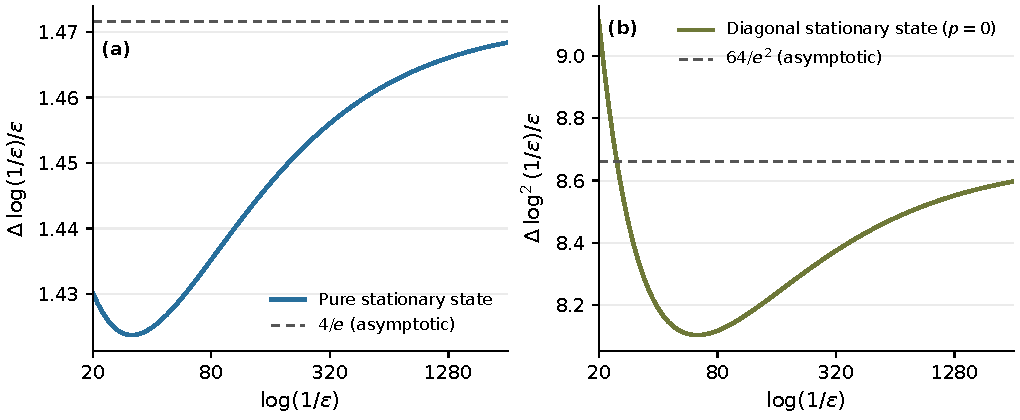
\includegraphics[width=\linewidth]{reset_convergence.pdf}
 \caption{Explicit attainable reset constructions, with achieved gain $\Delta=\eps-a$ and actual output error $\eps=P(0|1)$. (a) The pure-stationary-state family \eqref{eq:familyparams}--\eqref{eq:familyjump} approaches $4/e$ after logarithmic rescaling. (b) The diagonal-stationary-state family \eqref{eq:diag-jump}--\eqref{eq:diag-xstar}, with $p=0$, approaches $64/e^2$ after rescaling by $\log^2(1/\eps)$. Solid curves are evaluated for the explicit generators above; dashed lines show the asymptotic constants.}
 \label{fig:convergence}
\end{figure}


\section{Relation to the four-parameter family}\label{app:prior-family}

The family used for numerical boundary searches in Ref.~\cite{Shahbeigi2024} has
\begin{equation}\label{eq:prior-family}
 \begin{gathered}
 H_{\rm old}=X,\qquad
 J_{\rm old}=\sqrt\gamma\,\ket{\psi_o}\bra{\psi_i},\\
 \ket{\psi_j}=\binom{\cos\theta_j}{i\sin\theta_j},\qquad \gamma,t>0.
 \end{gathered}
\end{equation}
Its parameters have no physical upper bound. The numerical tolerance used in that search does not restrict this mathematical family.

For each fixed finite parameter choice of the pure-stationary-state construction,
\begin{equation}\label{eq:prior-pure-rankone}
 J=\sqrt{A+B}\ket u\bra e,\qquad
 \ket u=\frac{-\sqrt B\ket e+\sqrt A\ket g}{\sqrt{A+B}}.
\end{equation}
The vectors $u,e$ are real in the measurement basis. The unitary $S=\diag(1,i)$ preserves both preparation and measurement projectors and sends any normalized real vector to the form in \eqref{eq:prior-family}. Put $V_{\rm old}=S\ket u\bra eS^\dagger$. For $t_n\downarrow0$ and $\gamma_nt_n=A+B$, the old-family channels satisfy
\begin{equation}\label{eq:prior-pure-limit}
 \exp\!\left(-it_n[X,\cdot]+(A+B)\Diss[V_{\rm old}]\right)
 \longrightarrow \exp\!\left(\Diss[SJS^\dagger]\right).
\end{equation}
Continuity of the finite-dimensional matrix exponential proves inclusion of each such table in the old family's probability closure. This approximation is made at fixed $A,B,p$; the separate limit $L\to\infty$ subsequently approaches reset.

For the diagonal construction \eqref{eq:diag-jump}, $\tau=2/\log(1/\nu)>4\chi$ for sufficiently small $\nu$. The real jump then has a negative real eigenvalue $\xi$ satisfying
\begin{equation}\label{eq:prior-diag-shift}
 \begin{gathered}
 \xi^2+\sqrt B\,\xi+A\chi=0,\qquad
 J'=J-\xi I,\\
 H'=H+\frac{i\xi}{2}(J-J^\dagger).
 \end{gathered}
\end{equation}
This identity shift preserves the GKSL generator. Since $J'$ is nonzero, real, and singular, it has rank one. Moreover,
\begin{equation}\label{eq:prior-diag-hamiltonian}
 \begin{gathered}
 H'_{12}=ik',\\
 k'=\kappa_H-\frac{\xi}{2}(\sqrt A+\sqrt U)>0,\\
 SH'S^\dagger=k'X.
 \end{gathered}
\end{equation}
Write $J'=s\ket{u'}\bra{v'}$ with $s>0$ and real unit vectors. After the same phase change, choose the old-family duration $t=k'$ and jump rate $\gamma=s^2/k'$. Its integrated generator is exactly the transformed time-one generator of the diagonal construction. Thus this family lies in the prior ansatz itself for all sufficiently small $\nu$.

These transformations establish the stated relation to the prior family.

\section{Comparison of exclusion regions}\label{app:exclusions}\label{sec:exclusions}

To compare with the earlier analytic outer bound, denote the reset-side function in Theorem~1 of Ref.~\cite{Shahbeigi2024} by
\begin{equation}\label{eq:oldg}
 g_R(a)=(2-a)(2a+a^{1/10}).
\end{equation}
That theorem excludes tables when $a\le10^{-6}$, $\eps>g_R(a)$, and a second condition separating them from the swap endpoint holds. Near reset that second condition holds automatically. Since
$g_R(a)=2a^{1/10}[1+o(1)]$ is locally increasing, its inversion gives the necessary lower bound
\begin{equation}\label{eq:oldinverse}
 a\ge(\eps/2)^{10}[1+o(1)].
\end{equation}
This is a comparison derived from the earlier bound, not a claimed asymptotic formula for the true boundary.

For a direct open-region comparison, fix $C>4/e$ and choose $\eps_C>0$ so that Theorem~\ref{thm:main} implies $a\ge\eps[1-C/\log(1/\eps)]$ below this threshold. Every table in
\begin{equation}\label{eq:newwedge}
 \begin{split}
 \mathcal W_C=\bigl\{(a,1-\eps):\;&0<\eps<
 \min(\eps_C,e^{-4C},10^{-6}),\\
 &\eps/2<a<3\eps/4\bigr\}
 \end{split}
\end{equation}
is excluded by the present bound. None is excluded by the earlier theorem or its exchanged-coordinate version. Indeed, for $0<a<1$,
$g_R(a)>2a(2-a)>2a>\eps$, so the earlier reset condition fails; after exchanging the coordinates, the first coordinate is near one and fails its small-coordinate premise. Thus the improvement has nonzero area, without requiring a numerical boundary estimate.

\begin{thebibliography}{5}
\bibitem{Shahbeigi2024}
F.~Shahbeigi, C.~T.~Chubb, R.~Kukulski, {\L}.~Pawela, and K.~Korzekwa,
Quantum-embeddable stochastic matrices,
\href{https://doi.org/10.22331/q-2024-07-10-1404}{\emph{Quantum} \textbf{8}, 1404 (2024)}.

\bibitem{KorzekwaLostaglio2021}
K.~Korzekwa and M.~Lostaglio,
Quantum advantage in simulating stochastic processes,
\href{https://doi.org/10.1103/PhysRevX.11.021019}{\emph{Phys. Rev. X} \textbf{11}, 021019 (2021)}.

\bibitem{Benatti2024}
F.~Benatti, D.~Chru\'sci\'nski, and G.~Nichele,
Quantum versus classical $P$-divisibility,
\href{https://doi.org/10.1103/PhysRevA.110.052212}{\emph{Phys. Rev. A} \textbf{110}, 052212 (2024)}.

\bibitem{GKS1976}
V.~Gorini, A.~Kossakowski, and E.~C.~G.~Sudarshan,
Completely positive dynamical semigroups of $N$-level systems,
\href{https://doi.org/10.1063/1.522979}{\emph{J. Math. Phys.} \textbf{17}, 821--825 (1976)}.

\bibitem{Lindblad1976}
G.~Lindblad,
On the generators of quantum dynamical semigroups,
\href{https://doi.org/10.1007/BF01608499}{\emph{Commun. Math. Phys.} \textbf{48}, 119--130 (1976)}.

\end{thebibliography}
\end{document}

